\documentclass{standalone}
\usepackage{preset}
\begin{document}
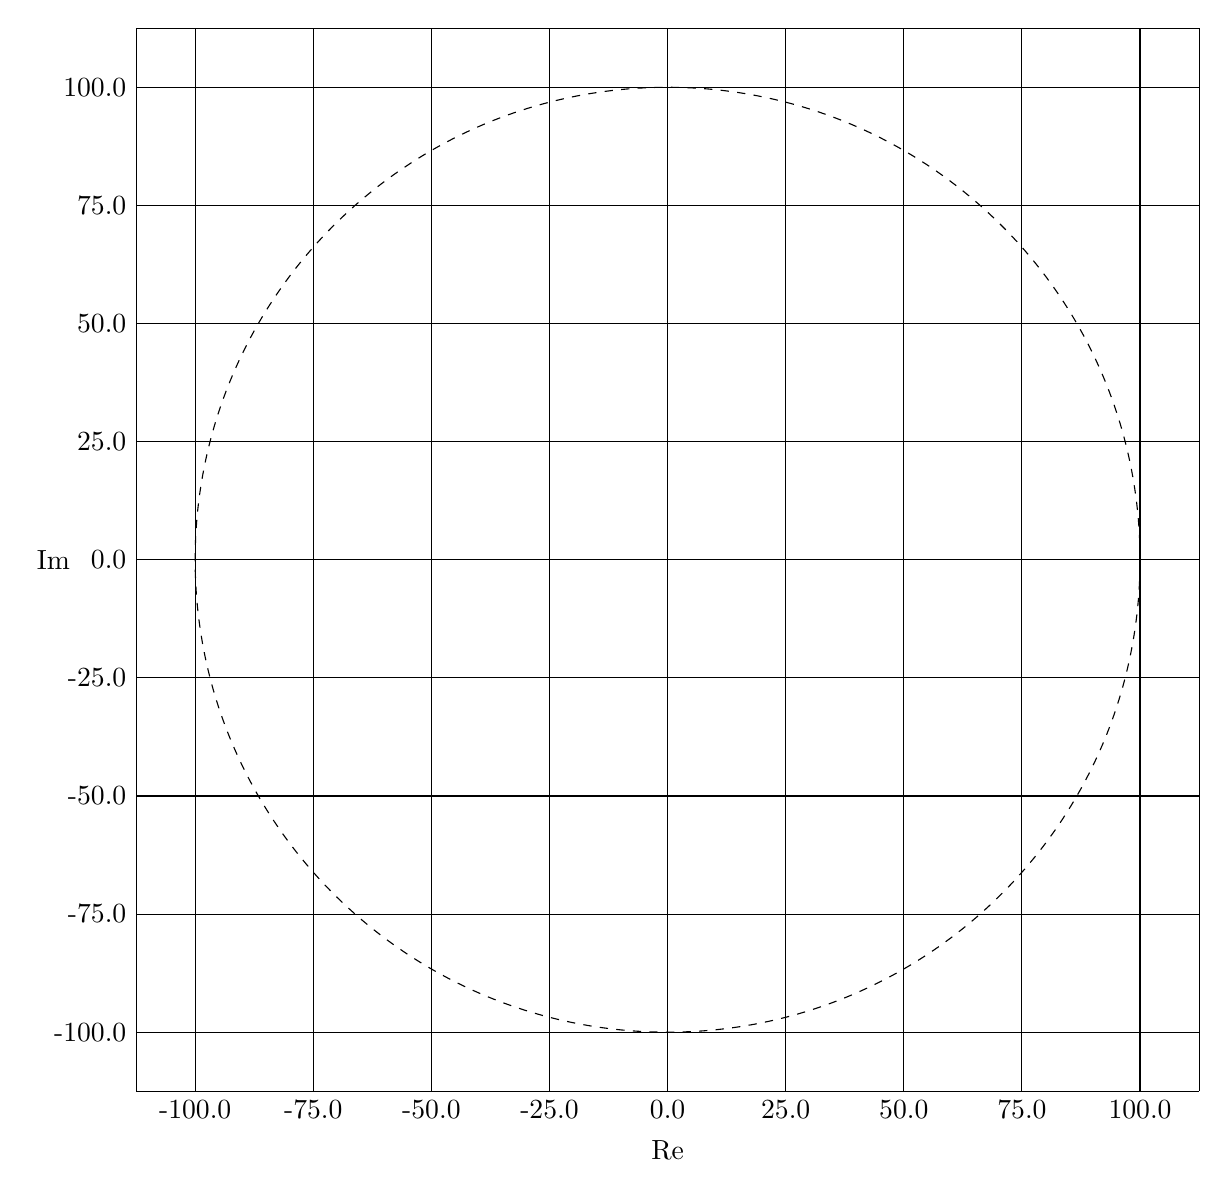
\begin{tikzpicture}[x=15mm,y=15mm]
	\foreach \i in {-4.5,-4,-3,-2,-1,0,1,2,3,4,4.5}{
		\draw(-4.5,\i)--(4.5,\i);
		\draw(\i,-4.5)--(\i,4.5);
	}
	\foreach \i in {-4,-3,...,4}{
		\pgfmathsetmacro{\val}{25*\i};
		\draw(\i,-4.5)node[below]{\val};
		\draw(-4.5,\i)node[left]{\val};
	}
	\draw(0,-5)node{Re};
	\draw(-5.2,0)node{Im};
	\draw[dashed](0,0)circle(4);
	\foreach \p in {({4*cos(112)},{4*sin(112)}),({4*cos(158)},{4*sin(158)}),({4*cos(-112)},{4*sin(-112)}),({4*cos(-158)},{4*sin(-158)})}{
		\draw\p node{$\cross$};
	}
\end{tikzpicture}
\end{document}
